\documentclass[30pt,a4paper]{article}
% Dokumenten Typ, titelseite, Schriftgröße, Seitenformat
\PassOptionsToPackage{dvipsnames}{xcolor}
% Füge neue Farben hinzu (standart 5 farben oder so)
\usepackage[utf8]{inputenc}
% Kodierung
\usepackage[T1]{fontenc}
% Umlaute
\usepackage[english]{babel}
% Eingebundene Sprachen
\usepackage{graphicx}
% Einbinden von Grafiken
\usepackage{wrapfig}
% Text um kleine Grafiken herumsetzen
\usepackage{amsmath}
\usepackage{amsfonts}
\usepackage{amssymb}
% Mathe Symbole und Commands
\usepackage{mathtools}
% Verbessert ams Packete von oben
\usepackage{nicefrac}
% Schönere Brüche
\usepackage{tikz}
\usepackage{circuitikz}
\usepackage{tikz-cd}
% Tikz Stuff
\usepackage{enumerate}
% Bessere Aufzählungen
\usepackage{cancel}
% z.B Durchstreichen von Sachen
\usepackage[hidelinks]{hyperref}
\usepackage{cleveref}
% Links und Referenzen innerhalb des Dokuments
\usepackage{tcolorbox}
% Wunderschöne Farbige Boxen mit Überschriften
\usepackage{caption}
% Erstellen von captions innerhalb einer Minipage
\usepackage[margin=1in]{geometry}
% Änderung der Gestaltung einer Seite (Überschreibt \documentclass)
\usepackage{placeins}
% Mit Hilfe von \FloatBarrier floats einschränken
\usepackage{booktabs}
% Bei Tabellen wird kann anstelle von \hline \toprule, \midrule und \bottomrule verwendet werden etc.
\usepackage{wasysym}
% Fügt eine Reihe von Symbolen wie Männlich Weiblich dazu
\usepackage{url}
% Füge Problemlos urls ein



\hbadness=99999 
% Löst ein Problem mit \hbox

\newenvironment{Dtabular}[2][1] {\def\arraystretch{#1}\tabular{#2}}
{\endtabular}

\title{
	\large Advanced Physics Lab	SS19 \\[4mm]
	\textbf{\LARGE Experiment: Short half lives
	} \\[4mm]
	(conducted on: 2.-3.9.2019 with Krzysztof Bozek) \\}
% Titel des Experiments
\author{Erik Bode, Damian Lanzenstiel \\ (Group 103)}
% Autoren

\begin{document}
	
	\begin{titlepage}
	\maketitle
	\vspace{2cm}
	\begin{abstract}
	In the short half life experiment, the half life of $^{57}$Fe in the $14.4$\,keV state is measured with the delayed coincidence method. As the source, the Cobalt Isotope $^{57}$Co is used.
	\end{abstract}
	\end{titlepage}
	\newpage
	
	\tableofcontents
	\newpage
	
	\section{Theory}
	\subsection{Radioactive Decays}
	Radioactive Decays are spontaneous processes in which a unstable atomic nucleus transforms into another lighter one while emitting other particles. Typical forms of radioactive decay are the alpha $\beta+$ and the $\beta-$decay.\\
	During the $\alpha-$decay a helium nucleus is emitted, reducing the atomic number by two. This form of decay is mainly found in heavy nucleus.\\ During the $\beta+$decay a proton transforms into a neutron and emits a positron as well as a electron-neutrino, reducing the atomic number by one.
	$$p\rightarrow n+e^++v_e$$
	On the other hand the $\beta-$decay is the reverse. It transforms a neutron into a proton and emits a electron and a electron-antineutrino. This decay increases the atomic number.
	$$n\rightarrow p+e^-+\bar{v}_e$$\\
	Another for the experiment important decay is the Electron Capture (EC) or $\epsilon-$decay. This one is similar to the $\beta+$decay since it also transforms a proton into a neutron. The difference being, that here the proton captures a electron to transform. The emitted particle is a electron-neutrino.
	$$p + e^- \rightarrow n + \bar{v}_e$$
	The captured electron is mostly from the K-shell while the resulting hole in the shell is filled by electrons from the L-shell. The remaining energy is either emitted through a X-ray photon or a Auger-electron. An Auger-electron is an electron that got the energy of an electron filling the vacancy left by electron in a lower state. The Auger-electron is therefore ejected. \\
	These decays are often accompanied by a $\gamma-$decays. When a decay occurs the daughter nucleus is mostly left in an exited state. It then decays into the ground state emitting $\gamma$-rays.\\
	Another Process similar to the $\gamma$-decay is the internal conversion (IC). Here the energy of a decay into a lower state is transmitted without radiation. That means no real photon is created to transport the energy. The energy is directly absorbed by another electron from the shell and ejected. The hole is filled similar to the one of EC by X-ray or Auger-electrons. 
	\subsection{Interaction between Matter and $\gamma-$Photons}	
 	When $\gamma-$photons and matter interact this happens mostly in 3 different ways depending on the atomic number of the atoms in the matter, as well as the Energy $E_\gamma$ of the photons.
 	\begin{enumerate}
 		\item Photoelectric effect:\\
 		The photoelectric effect happens when a photon is absorbed by an electron inside the matter. The energy carried by the photon is turned into kinetic energy and frees the electron. The vacancy is filled by electrons from higher shells and the energy is emitted by an Auger-electron or X-ray.\\
 		This effect appears mostly by $E_\gamma<200$\,keV and an atomic number around 50.
 		\item Compton scattering:\\
 		Unlike the photoelectric effect the photons are not absorbed by the electrons in the matter. They give up a part of their energy and scatter at the electron.\\
 		The Compton scattering happens by Energies in the range of $200$\,keV$<E_\gamma<5$\,MeV and a atomic number similar to the photoelectric effect.
 		\item Pair Production:\\
 		Pair production is an effect that appears by an energy $E_\gamma$ over the critical one of $1.022$\,MeV. When a $\gamma$-quantum gets into the electromagnetic field of a nucleus or electron it can be converted into an electron positron pair. 
 		$$\gamma \rightarrow e^- + e^+$$
 		To create this pair the energy of $1.022$\,MeV is needed this is also the reason the pair production can't happen if the photon has less energy. The remaining energy is given to the nucleus. The positron annihilates with an electron shortly after it's creation into two $\gamma$-rays with each half $0.511$\,MeV.
 	\end{enumerate}
 	\subsection{Energy Spectrum}
 	In the energy spectrum are a few areas of interest. \\
 	First of all their are the Photo-peaks. These are peaks which come into being when a photon gives its whole energy to the detector. This will happen during a photoelectric effect if the emitted x-Ray or auger electron also gets absorbed.\par
 	Another region of interest (ROI) could be the Escape-peak. Here the x-Ray emitted by an exited state dropping to back to the ground state leaves the detector without interaction. That means the Escape-peak will be shifted by the amount of energy that left the detector.\par
 	The next point is the Compton edge and spectrum. If the emitted photon only interacts with the detector only by Compton scattering, and leaves the detector only a part of the energy will be deposed. This energy will form the Compton-spectrum. For a scattering angle of $180$ the maximum amount of energy will be absorbed. This energy symbols the abrupt end of this spectrum and is called the Compton-edge.\\
 	Last but not least there is the Backscatter-peak happens through photons that get scattered at material outside of the detector and find their way back in where they get absorbed. That way they lose some energy depending on the material. This is way the peak is shifted by this amount from the position of the Photo-peak. 
 	\subsection{Methodology}
 	\ \\ 
 	\begin{wrapfigure}{l}{8cm}
 		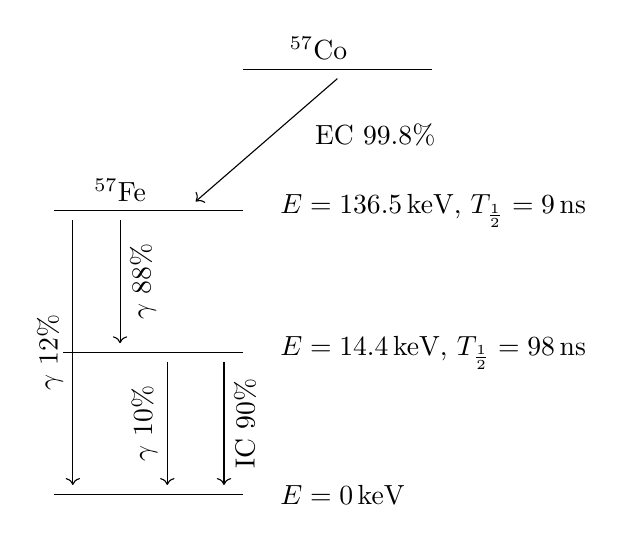
\begin{tikzpicture}[scale=1.2]
 		\draw (1,1.5) -- (1.8,1.5) node[above]{$^{57}$Co} -- (3,1.5);
 		\draw[->] (2,1.4) -- (0.5,0.1);
 		\node at (2.4,0.8) {EC $99.8\%$};
 		\draw (-1,0) -- (-0.3,0) node[above]{$^{57}$Fe} -- (1,0) node[right]{\quad$E=136.5$\,keV, $T_\frac{1}{2}=9$\,ns};
 		\draw (-0.9,-1.5) -- (1,-1.5) node[right]{\quad $E=14.4$\,keV, $T_\frac{1}{2}=98$\,ns};
 		\draw (-1,-3) -- (1,-3) node[right]{\quad$E=0$\,keV};
	 	\draw[->] (-0.8,-0.1) -- node[rotate=90,above]{$\gamma$ 	$12\%$} (-0.8,-2.9);
 		\draw[->] (0.2,-1.6) -- node[rotate=90,above]{$\gamma$ $10\%$}(0.2,-2.9);
 		\draw[->] (-0.3,-0.1) -- node[rotate=90,below]{$\gamma$ $88\%$} (-0.3,-1.4);
 		\draw[->] (0.8,-1.6) -- node[rotate=90,below]{IC $90\%$} (0.8,-2.9);
 		\end{tikzpicture}
 		\caption{\small Decay scheme for the cobalt isotope $^{57}$Co into $^{57}$Fe used into the experiment to measure the half-life of the $14.4$\,keV state of the Iron isotope.}
 		\label{CoDecay}
 	\end{wrapfigure}
 	\ \\ 
 	To measure the half-life of $^{57}$Fe we use the decay of the $^{57}$Co Isotope (see figure \ref{CoDecay}) $^{57}$Co decays by EC into an exited state of $^{57}$Fe. At this point it can either decay directly to the ground state emitting a $\gamma$-photon.\\
 	The more likely case with $88\%$ is, that it first goes to the wanted state of $14.4$\,keV by emitting a $\gamma-$ray. From this state it again has two options. With a $90\%$ probability we have an IC which we can't detect but there is also a $10\%$ chance that a $\gamma-$decay takes place.\\
 	\ \\
 	To measure the half-life it makes sense to use the method of delayed coincidence. For this kind of measurement we need to measure the time $\Delta t$ it takes for the $14.4$\,keV state to decay. The $\gamma$-photons connected to this state can be used to track the creation and the decay of the measured state and with that our time $\Delta  t$. This time is of interest since like the radioactive decay which is a stochastic process, it follows the eq.\ref{eq1}. \cite{delayC}
 	\begin{equation}
 		N(t)=N(0) e^{\frac{t}{\tau}}=N(0) *2^{\nicefrac{t}{T_\frac{1}{2}}}
 		\label{eq1}
 	\end{equation}
 	\begin{enumerate}
 		\item[•] $N(t)$: Number of existing nucleus at a given time.
 		\item[•] $N(0)$: Number of nucleus at the time zero.
 		\item[•] $\tau$: Mean life time of the decaying quantity.
 		\item[•] $T_\frac{1}{2}$: Half-life of the decaying quantity.
 	\end{enumerate}
	With that the amount of measured decays at certain times $\Delta t$ the half-life can be calculated. A problem that appears for the used decay is the rarity of the $\gamma$-ray with $14.4$\.keV. This one has only a $10\%$ chance of appearing and stopping our measurement. That would lead to a long dead time in which no new measurement can be taken. The problem is easily solved by using the rarer signal as the start of the measurement and stopping it with the $122$\,keV photon. Since there are also random coincidences which will distort the measurement a background measurement has to be made. This one can be subtracted from the real measurement.
 	
 	\subsection{$\gamma$-Ray Detection}
 	To detect the $\gamma$-rays two scintillators which react to the $\gamma$-photons exhibiting scintillation will be used. This again can be detected by a photomultiplier tube (PMT) and converts them into an electric pulse.\\
 	As scintillators organic and inorganic ones can be used. The main difference being the decay time of the emission centers and the luminous efficiency. If the half-life is bigger than $10^{-9}$\,s inorganic Naj(Tl)-scintillators are the choice since they have the higher luminous efficiency. For shorter times organic ones have to be used because of the shorter decay time.\\ For this experiment inorganic ones can still be utilized. The light from emitted can by light transmission bars to the PMTs. That way the loss will be minimized. \\ The PMT is used to generate an electric signal by using the photoelectric effect. The pulse is increased by using increasing the velocity of the electrons freed by the photons and using them to free even more electrons at the dynode. This process will be repeated till a useful signal is produced.
 	\section{Experimental Setup}
 	\subsection{Energy Spectra}
 	In the first part of the experiment the energy spectrum of $^{57}$Co and $^{241}$Am are measured. For this the setup in figure \ref{setup_ES} is used. Here the signals from the scintillator gets converted into an electric pulse and the Preamplifier (PA) provides a measurable signal. In the Main Amplifier (MA) the signal gets further amplified with low-noise. After this the pulse gets to the Multichannel Amplifier were it gets registered depending on the amplitude of the signal into a channel. This way a histogram can be formed. The output of the MA is for this measurement unipolar because only the amplitude of the signal is of importance. The spectra are needed to calibrate the MCA since a connection between known energies and the channel number can be made.\cite{Anleitung}
 	\begin{figure}[h]
 		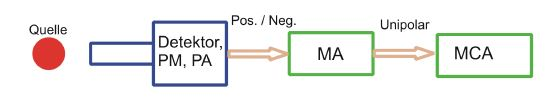
\includegraphics[scale=0.92]{Bilder/Circuit_ES}
 		\centering
 		\caption{\small Setup for the measurement of energy spectra with the MCA. \cite{Anleitung}}
 		\label{setup_ES}
 	\end{figure}
 	\subsection{SCA Thresholds}
 	In the next part of the experiment the energy windows for the Single Channel Analyser (SCA) have to be set. One have to be set to filter out $122.1$\,keV photons and the other one to filter the $14.4$\,keV ones out. For this the setup in figure \ref{setup_EW} is used. The Linear Gate in the setup only lets through a signal only when two signals one at the input and on at the enabler arrive at the same time. That way we can precisely set the energy window at the SCA. By moving the upper and lower threshold of the window, pulses with amplitudes outside of the thresholds are stopped and with that the other signal is stopped at the gate as well. By watching the histogram created by the MCA the thresholds can be set to the correct energy levels. \cite{Anleitung}
 	\begin{figure}[h]
 		\includegraphics{Bilder/Circuit_ES_calib}
 		\centering
 		\caption{\small Setup for the calibration of the energy windows to filter out the photons with correct energies. \cite{Anleitung}}
 		\label{setup_EW}
 	\end{figure}\\
 	\FloatBarrier
 	\subsection{Delayed Coincidences}
 	The setup in figure \ref{setup_DC} is used to make the measurement of delayed coincidences. In this setup the two sides of the detectors are connected to the calibrated SCAs. The TAC takes a start and a stop signal and creates a signal with an amplitude proportional to the time between the input signals. Since the measurement is started with the later $14.4$\,keV photon the earlier photon needs to be delayed so that it can stop the measurement.\cite{Anleitung}
 	\begin{figure}[h]
 		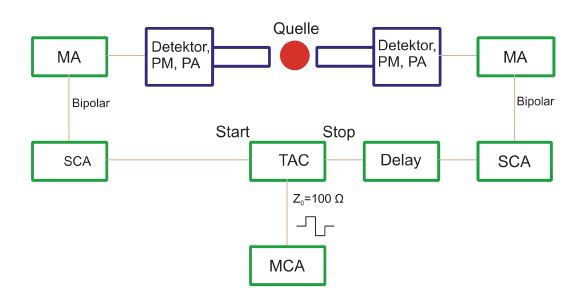
\includegraphics{Bilder/Circuit_DC}
 		\centering
 		\caption{\small Setup for the measurement with the method of delayed coincidences. \cite{Anleitung}}
 		\label{setup_DC}
 	\end{figure}\\
 	\subsection{TAC Calibration}
 	Last but not least the TAC needs to be calibrated. For this the setup in figure \ref{setup_TC} will be used. With this the constant of proportionality between the delay and the channel number of the MCA can be calculated. \cite{Anleitung}
 	\begin{figure}[h]
 		\includegraphics{Bilder/Circuit_DC_calib}
 		\centering
 		\caption{\small Setup for the calibration of the TAC. \cite{Anleitung}}
 		\label{setup_TC}
 	\end{figure}\\
 	\section{Conduction of the Experiment}
 	First of all the $^{141}Am$ isotope was put into the detector. Directly after the PA and the MA were connected to an oscilloscope. Here the signals of both could be compared like in figure \ref{Bi}.\\
 	After this, the MCA was connected like in figure \ref{setup_ES}. The MCA was also connected to the interface from which the measurement of the energy spectra can be started. With the $^{141}Am$ source one measurement with each scintillator was made. These can be used to make the energy calibration of the MCA.\par
 	After this measurement the  $^{141}Am$ source was switched with the $^{57}$Co source. Here four different spectra were taken, two for both detectors with different sides of the sample. Here the LLD value needed to be tuned a bit to decrease a noise signal at the low energy range. With these information the best combination of side of the sample and scintillator was chosen for the different energies. With this set the calibration of the energy windows could be started. For this the layout in figure \ref{setup_EW} was used. First the window was opened completely so the whole spectrum, which was measured before could be seen. Than the thresholds at the SCA were slowly adjusted so that only one peak of the needed energy could be seen on the computer. The Peaks in the threshold calibration can be seen in figure \ref{low} and \ref{high}\par
 	After both SCAs were configured the actual measurement seen in figure \ref{setup_DC} was set up. For the delay we choose the highest of $196$\,ns to get as much of the exponential curve as possible. After running a test the main measurement was started with a timer of 15 hours. Since the measured spectrum had a big part with only random coincidences this can be used instead of another measurement for the random coincidences. At last the calibration for the TAC was done by using the setup of figure \ref{setup_TC}. Here different delays were set and the corresponding channel were noted.
 	\section{Analysis}
 	\subsection{Energy Calibration}
 	To calibrate the MCA the decay of the Americium is used since it has clear visible Photo-peaks with known energies. To get the position of the peaks three Gaussian peaks are fitted on the curves. For the fits the python package \verb|scipy.optimize.curve_fit|\cite{SciPy_Opti} was used. For the $59.5$\,keV peak the equation \ref{eq6} was used. 
 	\begin{equation}
 	f(x)=Ae^{-\frac{x-\mu}{2\sigma^2}}+C \label{eq6}
 	\end{equation}
 	In figure \ref{Am3peak} the two peaks can be seen. For the other two peaks which are pushed together, two added Gaussian curves in the form of equation \ref{Am12peak} are used.
 	\begin{equation}
 	f(x)=Ae^{-\frac{x-\mu}{2\sigma^2}}+A_2e^{-\frac{x-\mu_2}{2\sigma_2^2}}+C \label{Am12peak} 
 	\end{equation}
 	These fits are given in figure \ref{ASL} and \ref{ASR}. With the value of the three different $\mu$ we get the position of the maximums.\\
 	\begin{table}[h]
 	\begin{Dtabular}[1.1]{|c|c|c|c|}
 		\hline
 		&$59.5\,$keV&$33.2\,$keV&$26.3\,$keV \\
 		\hline
 		Right Scintillator $\mu$&$120.61\pm0.23$&$191.25\pm0.29$& $419.53\pm0.023$\\
 		\hline
 		Left Scintillator $\mu$&$123.92\pm0.30$&$179.91\pm0.28$ &$372.83\pm0.022$\\
 		\hline
 	\end{Dtabular}
 	\centering
 	\caption{Positions of the different energy peaks of the right and left scintillator.}
 	\label{EnCalib}
 	\end{table}\\
 	These values can be plotted as a line which gives for every channel the corresponding energy. $R^2$ is the coefficient of determinate and n the channel number. 
 	\begin{equation}
	f(x)_{Right}=(0.1120\pm 0.0033)\,\nicefrac{\text{keV}}{n}*x+ (12.3\pm0.9)\,\text{keV} \qquad R^2=0.9991 \label{eqRC}
 	\end{equation}
	\begin{equation}
	f(x)_{Left}=(0.1341\pm 0.0023)\,\nicefrac{\text{keV}}{n}*x+ (9.4\pm0.5)\,\text{keV} \qquad R^2=0.9996 \label{eqLC}
	\end{equation}
	The fits can be seen in figure \ref{EnergieCalib}.
 	\subsection{Analysis of the Signal Shapes}
 	\begin{figure}
 		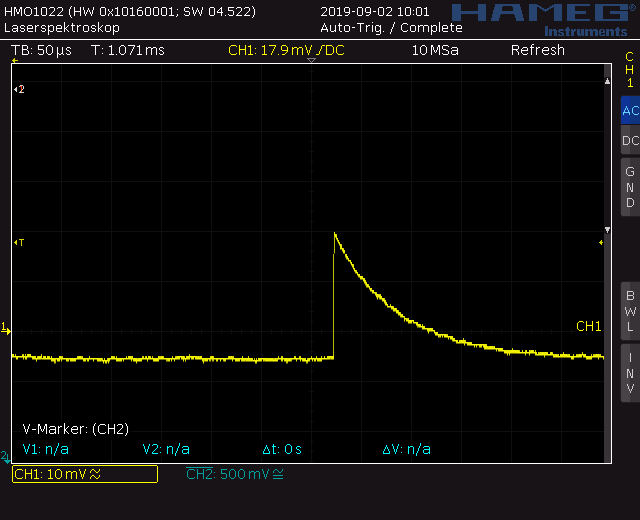
\includegraphics[scale=0.42]{Bilder/OsziPA}
 		\centering
 		\caption[Preamplifier Signal]{Signal of the PA measured with an oscilloscope.}
 		\label{PA}
 	\end{figure}
 	\begin{figure}
 		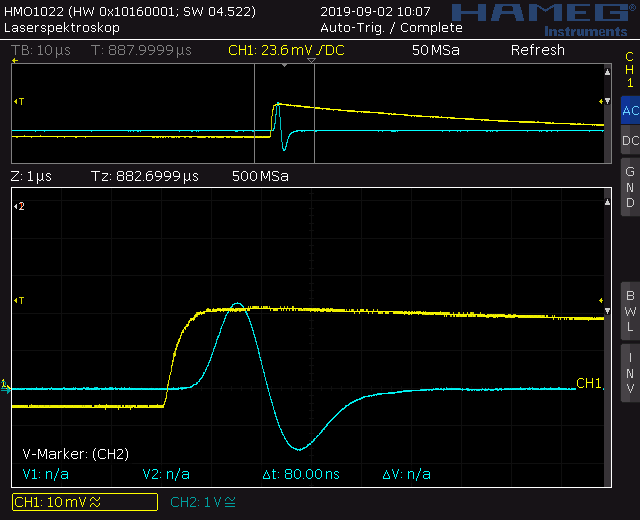
\includegraphics[scale=0.42]{Bilder/OsziBipolar}
 		\centering
 		\caption[Bipolar Signal]{Bipolar signal output of the MA compared to the signal coming from the PA. Measured with an oscilloscope. In yellow the signal of the PA. In Blue the signal of the MA.}
 		\label{Bi}
 	\end{figure}
 	\begin{figure}
 		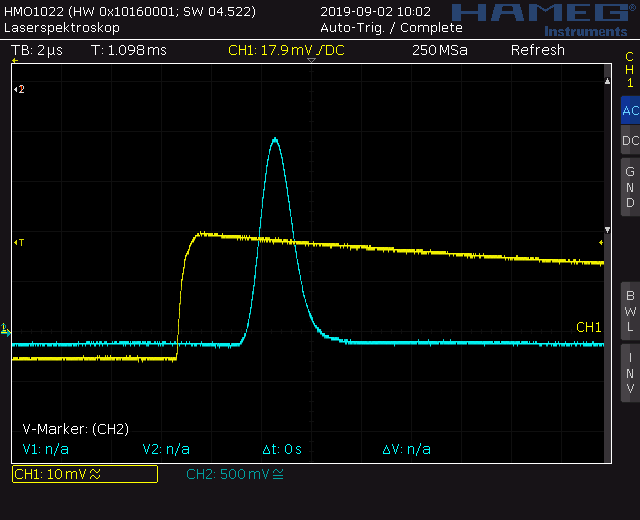
\includegraphics[scale=0.42]{Bilder/OsziUnipolar}
 		\centering
 		\caption[Unipolar Signal]{Unipolar signal output of the MA compared to the signal coming from the PA. Measured with an oscilloscope. In yellow the signal of the PA. In Blue the signal of the MA.}
 		\label{Uni}
 	\end{figure}
 	\begin{figure}
 		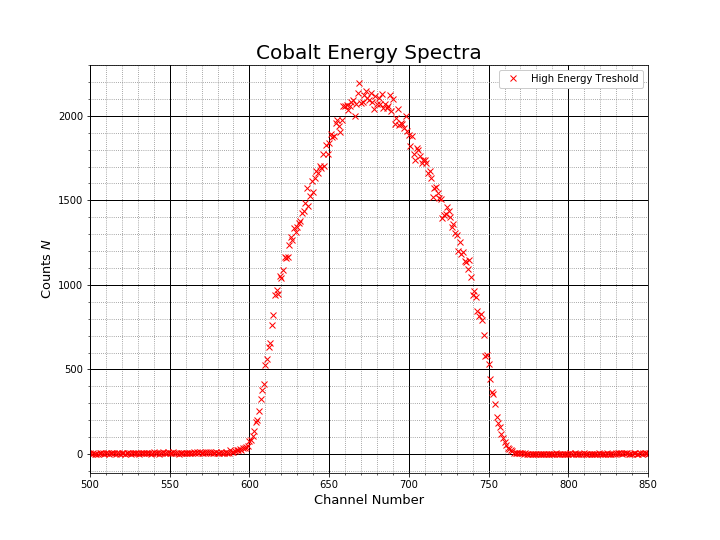
\includegraphics[scale=0.42]{Bilder/HighThresh}
 		\centering
 		\caption[High Energy Threshold]{Peak during the high energy threshold calibration of the SCA. It's around the expected energy of the $122.1$\,keV photon.}
 		\label{high}
 	\end{figure}
 	\begin{figure}
 		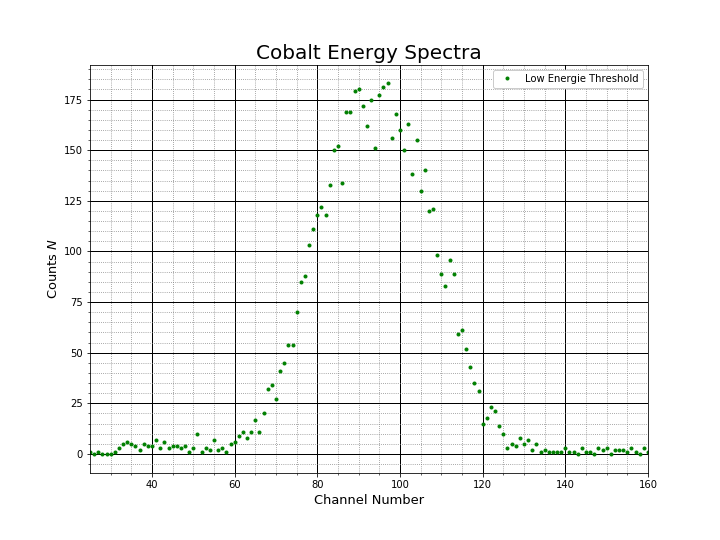
\includegraphics[scale=0.42]{Bilder/LowThresh}
 		\centering
 		\caption[Low Energy Threshold]{Peak during the low energy threshold calibration of the SCA. It's around the expected energy of the $14.4$\,keV photon.}
 		\label{low}
 	\end{figure}
 	In figure \ref{PA} we see the signal coming from the PA output of the detector. The signal reaches almost instantaneously its peak and than drops slowly down to the ground level. If we compare this signals with the one coming from the MA we can see that they are more Gaussian like and the beginning of the signal is a bit shifted to the left. In figure \ref{Bi} the maximum of the blue signal is only a bit higher than the signal of the PA but its obvious that we have a bipolar signal. It is also notable that the ground level of the MA is higher than the one of the PA. In figure \ref{Uni} this is the same but we see that the maximum amplitude of the MA signal is much higher than the one of the PA and we have a bell shaped signal. Comparing right and left slope of the MA curves with each other we notice that here the left side has a bit sharper increase than the right side of the signal.
 	\subsection{Analysis of the Energy Spectra}
 	\subsubsection{Americium Spectra}
 	Looking at figure \ref{AS} we see that the two spectra are shifted against each other. It is likely that the scintillators have a different amplification which causes this shift. Because of this two different energy calibrations are needed. \par
	Looking at the spectra we see mainly the three Photo-peaks of the decays we expect. The positions of other regions of interest (ROI) are noted in the table \ref{ROIs1}
	\begin{table}[h]
		\begin{Dtabular}[1.1]{|c|c|c|c|}
			\hline
			ROI&Expected Energy [keV]&Right Channel&Left Channel\\
			\hline
			Escape Peak of $59.5$\,keV&$31.5$&$171\pm10$&$165\pm5$\\
			\hline
			Escape Peak of $26.3$\,keV&-&-&-\\
			\hline
			Escape Peak of $33.2$\,keV&-&-&-\\
			\hline
			Compton Edge of $59.5$\,keV&$11.23$&$-10\pm8$&$14\pm4$\\
			\hline
			Compton Edge of $26.3$\,keV&$2.45$&$-88\pm9$&$-52\pm4$\\
			\hline
			Compton Edge of $33.2$\,keV&$3.82$&$-76\pm9$&$-42\pm4$\\
			\hline
		\end{Dtabular}
		\centering
		\caption{Points of interest for the scintillators. To calculate the channel equation \ref{eqRC} for the right side and equation \ref{eqLC} for the left side is used. The equations are tuned for the different scintillators. Left Channel gives the positions of the two spectra of the left one. The column Right Channel gives the position for the right scintillator. The - means that the peak ether cant exist in the spectrum.}
		\label{ROIs1}
	\end{table}
	To calculate the Escape Peak $28$\,keV were deducted from the Photo-peaks energy since this is the energy between the K and L shall in this experiment. To calculate the energy of the Compton edge equation \ref{comtonedge} was used.\par
	\begin{equation}
		E_{Compton}=E_{\text{Photon}}-\frac{E_{\text{Photon}}}{1+\frac{2E_{\text{Photon}}}{E_{\text{Electron}}}} \label{comtonedge}
	\end{equation}
	Looking at these it can be expected to see an Escape Peak of the $59.5$\,keV peak and its Compton Edge. The Reason we don't see them is that our Escape Peak is overshadowed by the Photo Peak of our $33.2\,$keV Photon. For the Compton Edge its possible that our energies are to low for it to happen often enough that it would get visible since the Compton scattering happens mostly in the range of $200\,$keV to $5\,$MeV.
	\subsubsection{Cobalt Spectra}
	The cobalt spectra was measured four times and all four spectra can be seen in figure \ref{4cobaltspectra}. Since the two spectra where the screw of the source was turned to the scintillator are much lower, these are separate in figure \ref{2cobaltspectra}. Looking at the figures we can clearly see the $122.1\,$keV peaks. But in this peak there is also hidden the in theory smaller, duo to its lower probability, $136.5$\,keV peak. These are similar to the $26.3\,$keV and $33.2$\,keV peaks very close to each other. That's why the $136.5$\,keV Photo-peak is hidden in the big peak at the right side of the spectrum. It is also visible that depending on which sides of detector are here also shifted against each other. Notable as well is that there is a smaller shift depending on the side of the source. So the spectra measured with the screw side are a bit sifted to the left. In the table \ref{ROIs2} the positions of certain expected regions are listed. The Compton Edge was calculated like in the Americium Spectrum before with equation \ref{comtonedge}.\par
	\begin{table}[h]
		\begin{Dtabular}[1.1]{|c|c|c|c|}
			\hline
			ROIs&Expected Energy [keV]&Right Channel&Left Channel\\
			\hline
			Photo Peak of $136.5$\,keV&$136.5$&$1107\pm34$&$947\pm17$\\
			\hline
			Photo Peak of $122.1$\,keV&$122.1$&$979\pm30$&$840\pm15$\\
			\hline
			Photo Peak of $14.4$\,keV&$14.4$&$18\pm8$&$37\pm4$\\
			\hline
			Escape Peak of $136.5$\,keV&$108.5$&$857\pm26$&$738\pm13$\\
			\hline
			Escape Peak of $122.1$\,keV&$94.1$&$729\pm23$&$631\pm12$\\
			\hline
			Escape Peak of $14.4$\,keV&-&-&-\\
			\hline
			Compton Edge of $136.5$\,keV&$11.23$&$313\pm12$&$284\pm6$\\
			\hline
			Compton Edge of $122.1$\,keV&$2.45$&$242\pm11$&$224\pm6$\\
			\hline
			Compton Edge of $14.4$\,keV&$3.82$&$-103\pm9$&$-64\pm5$\\
			\hline
		\end{Dtabular}
		\centering
		\caption{Expected positions of certain regions of interest in the cobalt spectrum. The channels were calculated out of the expected energies with the equations \ref{eqLC} and \ref{eqRC}. The equations are tuned for the different scintillators. Left Channel gives the positions of the two spectra of the left one. The column Right Channel gives the position for the right scintillator. The - means that the peak ether cant exist in the spectrum.}
		\label{ROIs2}
	\end{table}
	\begin{figure}[h]
		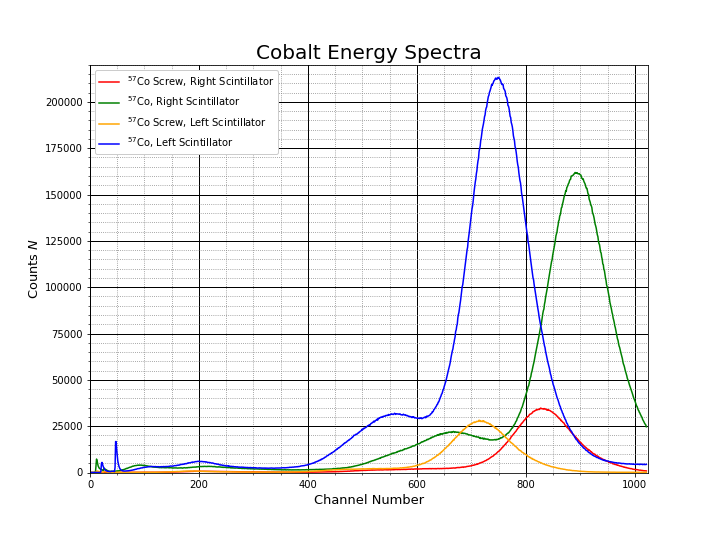
\includegraphics[scale=0.5]{Bilder/Cobalt_Energy_Spectra1}
		\centering
		\caption{Energy Spectra of Cobalt with both sides of the detector and sides of the source.}
		\label{4cobaltspectra}
	\end{figure}
	Comparing the expected positions to the measured ones we see that these don't align to well. For example is the expected position of the $136\,$keV Photo Peak outside of our measured spectrum for the right scintillator while left one is at the position were we see the right peak in figure \ref{4cobaltspectra}. Since it is unlikely that those peaks in the figure aren't the $122.1$\,keV peaks its possible that our calibration isn't very precise. The reason for this may be that there is a systematic error that wasn't considered which shifted the cobalt spectra or the americium spectra into one direction. If we consider this its very likely that the peaks closest to the $122.1$\,keV peaks are the $108.5\,$keV and $94.1\,$keV Escape Peaks because they are expected to be quite close to the main peaks. The Compton Edge is very likely not visible since the chance for Compton scattering is to low because of the low energy levels. At channel number 200 we see a peak which might be a backscatter peak which originates from photon that lost energy outside of the scintillator can got back were they were absorbed. The little increase after this is what we expected to be the  area of the $14.4\,$keV peak. Since the calibration isn't reliable we can't be sure of it. The low count rates at this part of the spectrum might come from the increase in the lower level discriminator (LLD) value during the experiment. Since there was an unrealistic high count rate at the lower energy level it was increased and it also affects the count rate of the region were the $14.4$\,keV photon is expected to be. The high count rate probably comes from electronics. 
	\begin{figure}[h]
		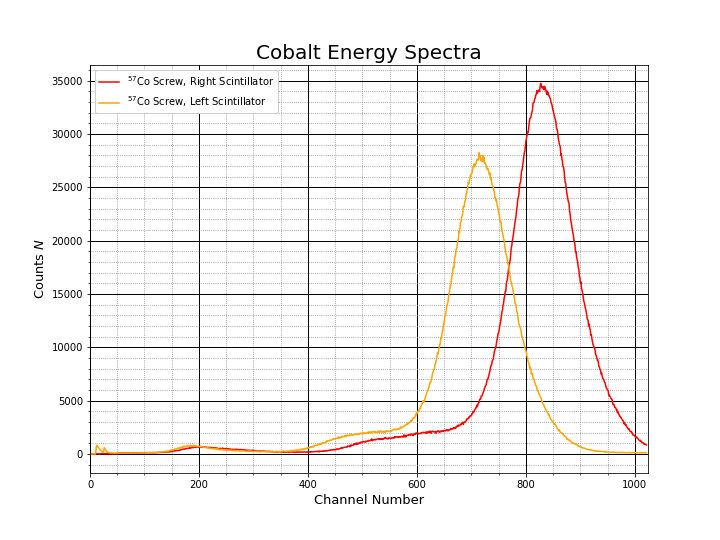
\includegraphics[scale=0.5]{Bilder/Cobalt_Energy_Spectra2}
		\centering
		\caption{Energy Spectra of Cobalt of the two less visible peaks duo to lower radiation from the side of the screw.}
		\label{2cobaltspectra}
	\end{figure}
	\begin{figure}[h]
		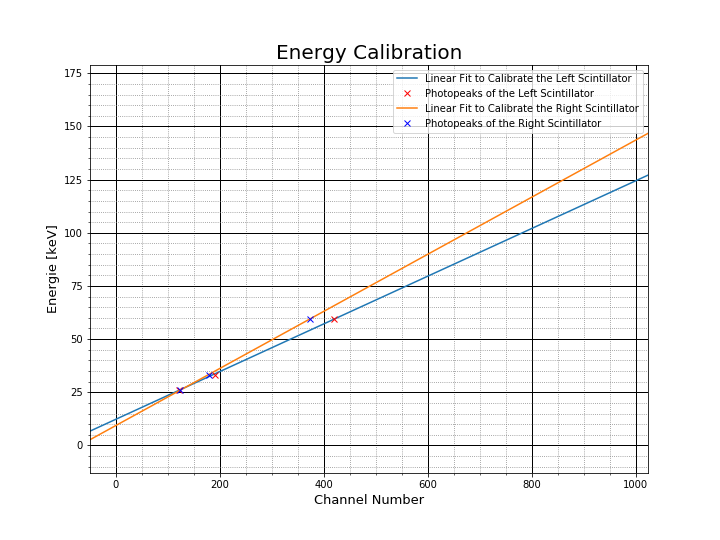
\includegraphics[scale=0.5]{Bilder/EnergyCalib}
		\centering
		\caption{Calibration curves for the energy calibrations.}
		\label{EnergieCalib}
	\end{figure}
 	\begin{figure}[h]
 		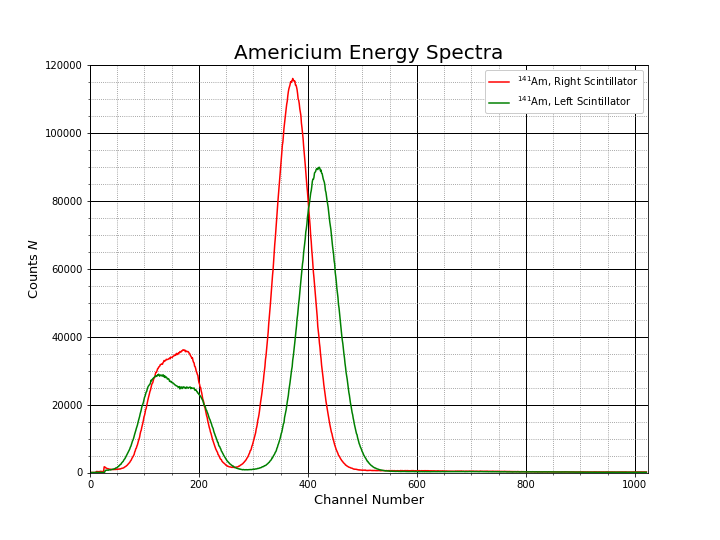
\includegraphics[scale=0.5]{Bilder/Americium_Energy_Spectra}
 		\centering
 		\caption[Americium Spectra]{Measured Americium Energy Spectra. The green curve is the measurement with the left scintillator while the red one is the scintillator of the right detector side.}
 		\label{AS}
 	\end{figure}
 	\begin{figure}[h]
 		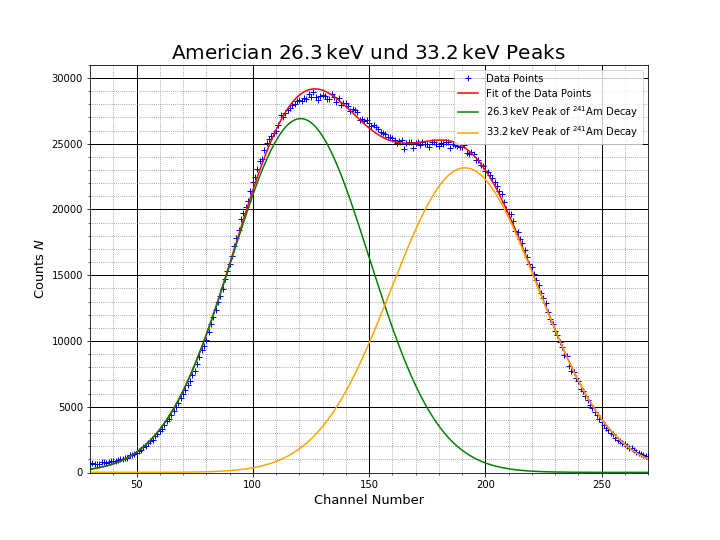
\includegraphics[scale=0.5]{Bilder/kleine_Peaks2}
 		\centering
 		\caption[Americium Spectra Double Peak Left Detector Side]{Measured Americium Energy Spectra of the $26.3$\,keV and $33.2$\,keV double peak with fits of the split peaks. Spectrum of the left scintillator.}
 		\label{ASL}
 	\end{figure}
 	\begin{figure}[h]
 		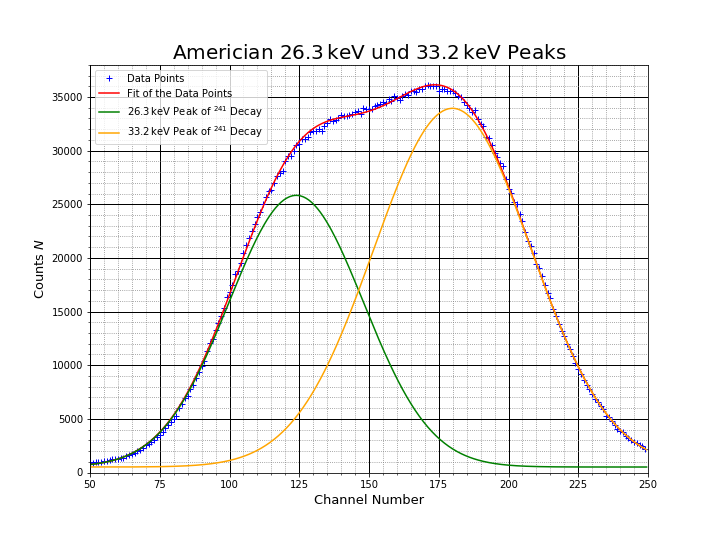
\includegraphics[scale=0.5]{Bilder/kleine_Peaks1}
 		\centering
 		\caption[Americium Spectra Double Peak Right Detector Side]{Measured Americium Energy Spectra of the $26.3$\,keV and $33.2$\,keV double peak with fits of the split peaks. Spectrum of the right scintillator.}
 		\label{ASR}
 	\end{figure}
 	\FloatBarrier
 	\subsection{Analysis of the delayed coincidences measurement}
 	\subsubsection{Time calibration}
 	To correctly compute the half-live of the $14.4$\,keV state of $^{57}$Fe, the conversion of time difference to the channels in the MCA is determined. 
 	The data collected for this purpose is found in the appendix. 
 	The channel and delay pairs were plotted and a unweighted linear model of first
 	order was fitted to the data. The plot is shown in figure \ref{time_cal_plot}.
 	The fitted linear model had the form of $n(\Delta t) = m \cdot \Delta t + c$. To calculate the parameters of the fit the python package \verb|scipy.optimize.curve_fit|\cite{SciPy_Opti} was used.	The fitted parameters were:
 	\begin{eqnarray}
 	m = (1.2 \pm 0.007)\frac{1}{\textrm{ns}} \\
 	c = (-21.5 \pm 0.7)
 	\end{eqnarray}
 	The error for the time was estimated to be $\pm 0.5\,\textrm{ns}$, which is too small
 	to be visible in the graphic.
 	This parameters were used to compute the time corresponding to each channel using 
 	formula \ref{chn_to_time}. $x_{\text{cal}}$ represents the calibrated value, $x_{\text{norm}}$ the original value.
 	
 	\begin{equation}
 	x_{\text{cal}} = \frac{x_{\text{norm}}-c}{m}
 	\label{chn_to_time}
 	\end{equation}
 	
 	\begin{figure}[h]
 		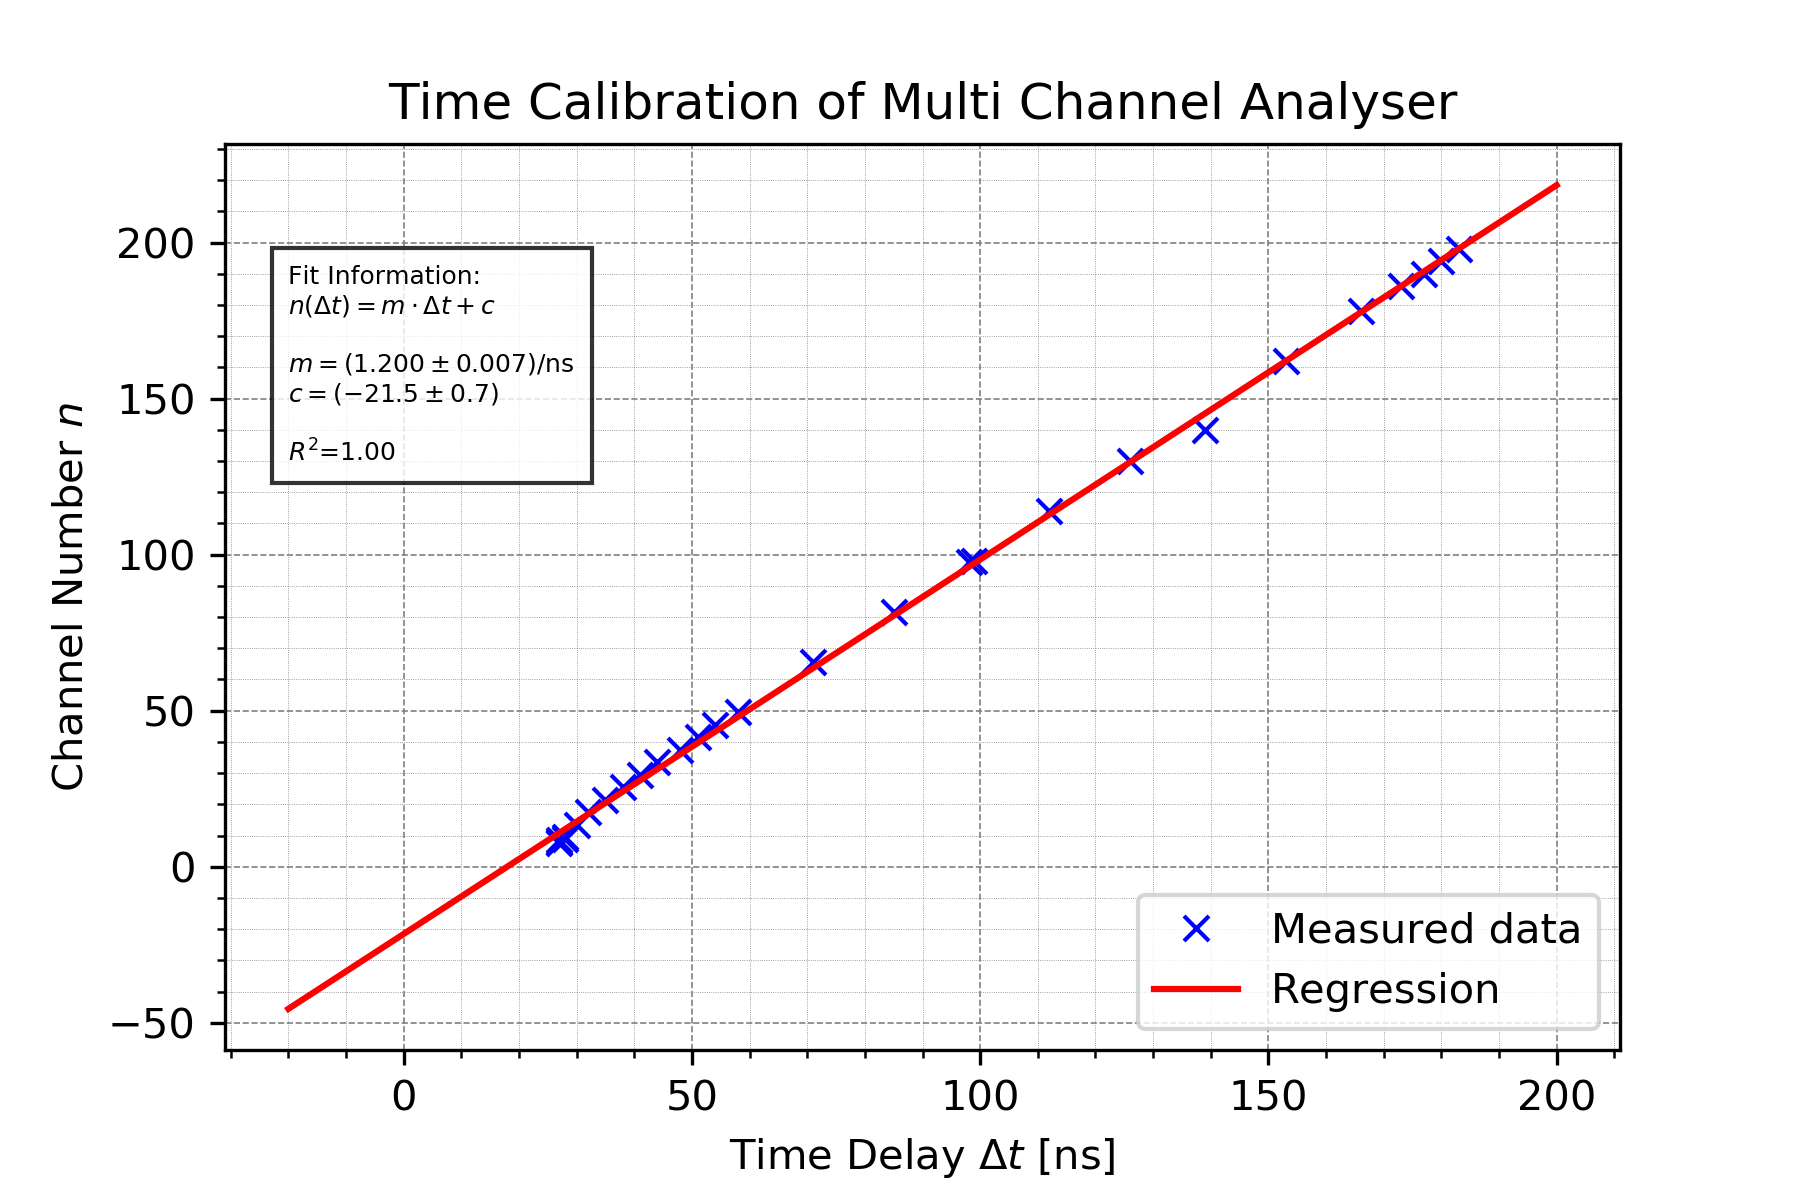
\includegraphics{Bilder/time_cal}
 		\centering
 		\caption{\small Plot of the datapoints of the time calibration and the linear fit of them. The errors are too small to be visible in the graphic.}
 		\label{time_cal_plot}
 	\end{figure}
 	
 	\subsubsection{Analysis on linear scale}
 	For the analysis in the linear scale, two ranges of the data set were chosen.
 	One	was used for the background compensation, the other one for the exponential fit.
 	For a visual representation and the exact value ranges, see figure \ref{raw_plot}.
 	The error on the counts is, because a poisson distribution was assumed, computed by
 	equation \ref{poisson_error}. $s_{\text{counts}}$ is the error for the counts of a channel, $n$  the actual counts of the same channel. All errors were calculated for each channel individually.
 	\begin{equation}
 	s_{\text{counts}}=\sqrt{n}
 	\label{poisson_error}
 	\end{equation}
 	
 	
 	\begin{figure}[h]
 		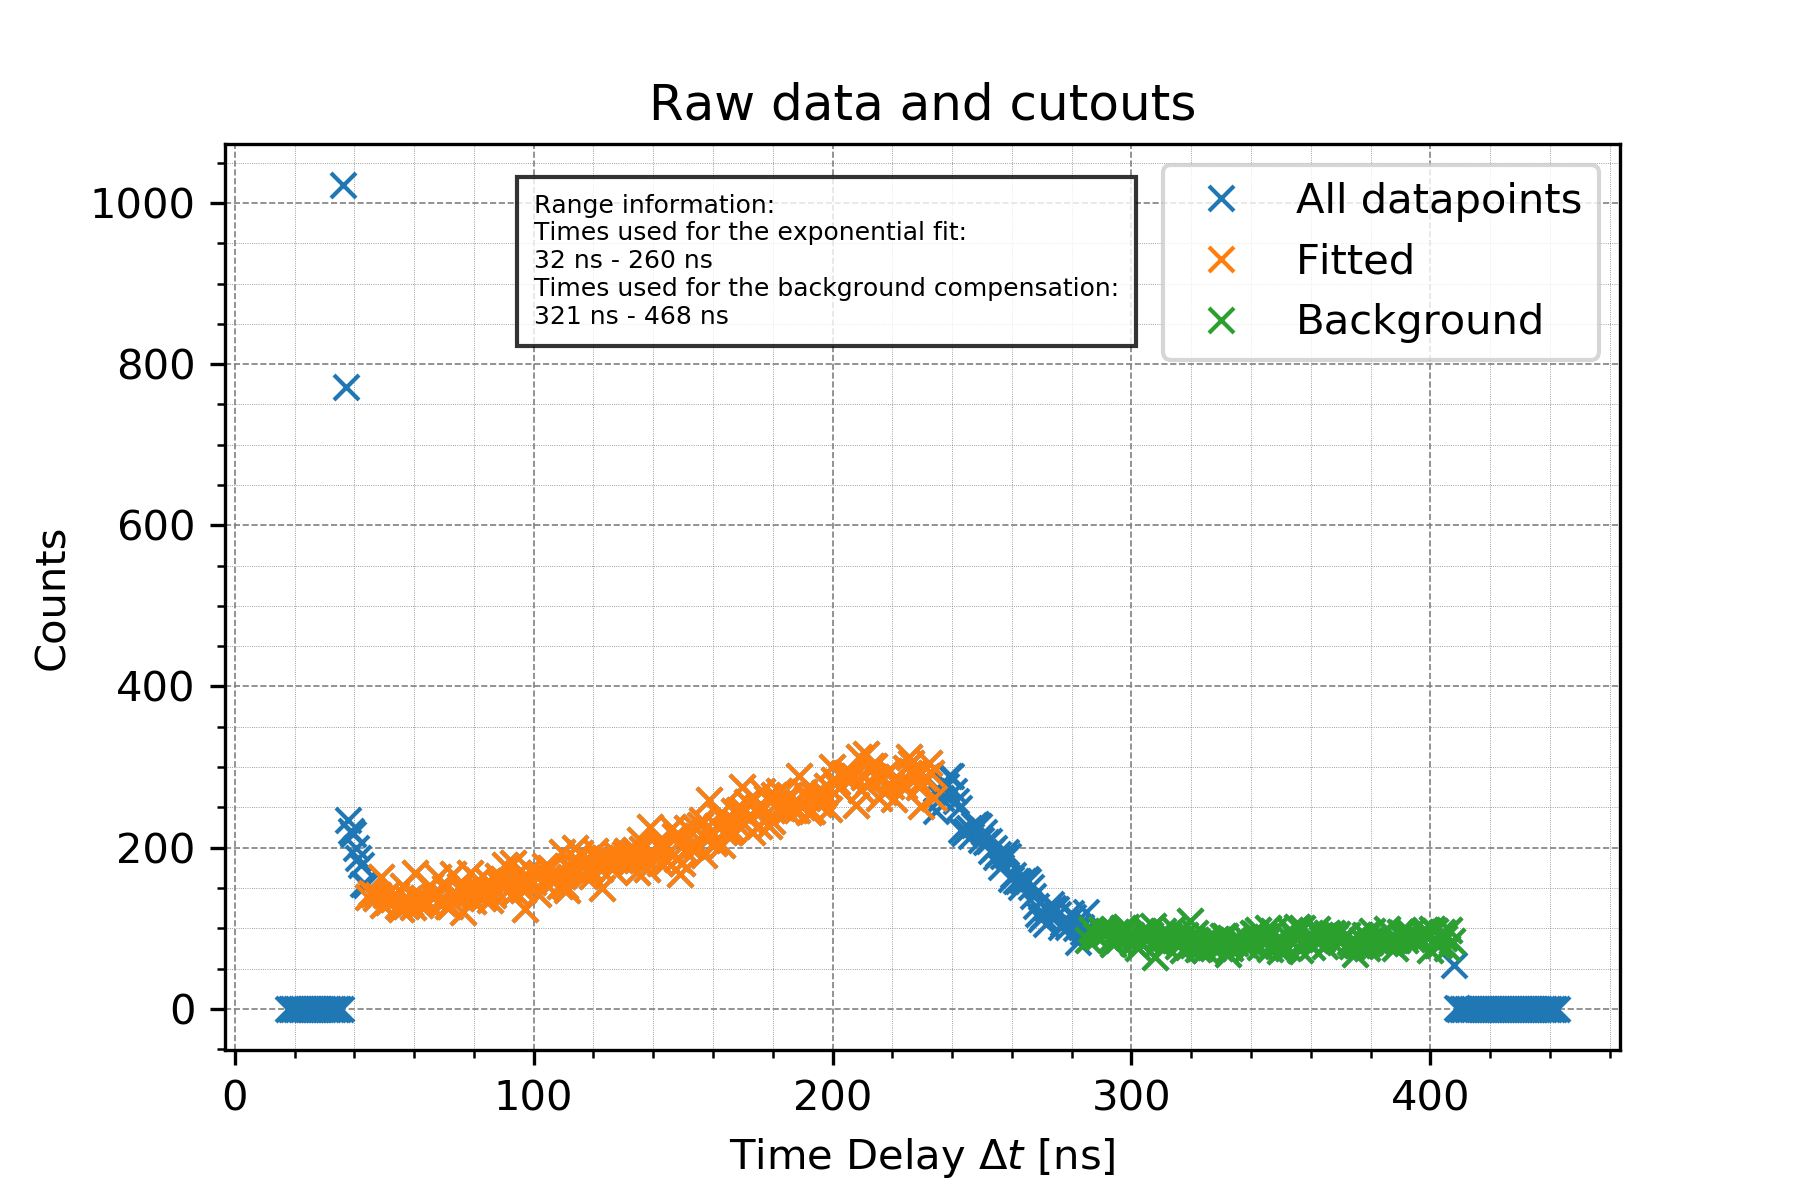
\includegraphics{Bilder/raw_ranges}
 		\centering
 		\caption{\small Plot of the datapoints with corrected time. The ranges of the data used for each different regression are marked in the graphic. The start and endpoints for each range are also given.}
 		\label{raw_plot}
 	\end{figure}
 	
 	As the next step a curve, analog to the one used for the time calibration, was
 	fitted to the range designated for the background compensation. A visual
 	representation of this fit is given in figure \ref{bckgnd_fit}. This fitted curve
 	was then subtracted from all the datapoints, as a mean to reduce the influence of
 	random background coincidences. The reason why the green part in figure \ref{raw_plot} can be used is that for the part of our measurement the random coincidences is almost flat. This is due to the fast decay of $9ns$ of our $136.5$\,keV state. Since it decays so fast the measurement takes part in the flat area of the background. To get the curve for the background we fit the Data Points using the python package \verb|scipy.optimize.curve_fit| \cite{SciPy_Opti}.
 	The parameters for the curve in form of $f(x)=m\cdot x+c$ are:
 	
 	\begin{equation*}
 	m = (-0.015 \pm 0.020)\frac{1}{\textrm{ns}}
 	\end{equation*}
 	$$c = (92 \pm 7)$$
 	
 	
 	
 	\begin{figure}[h]
 		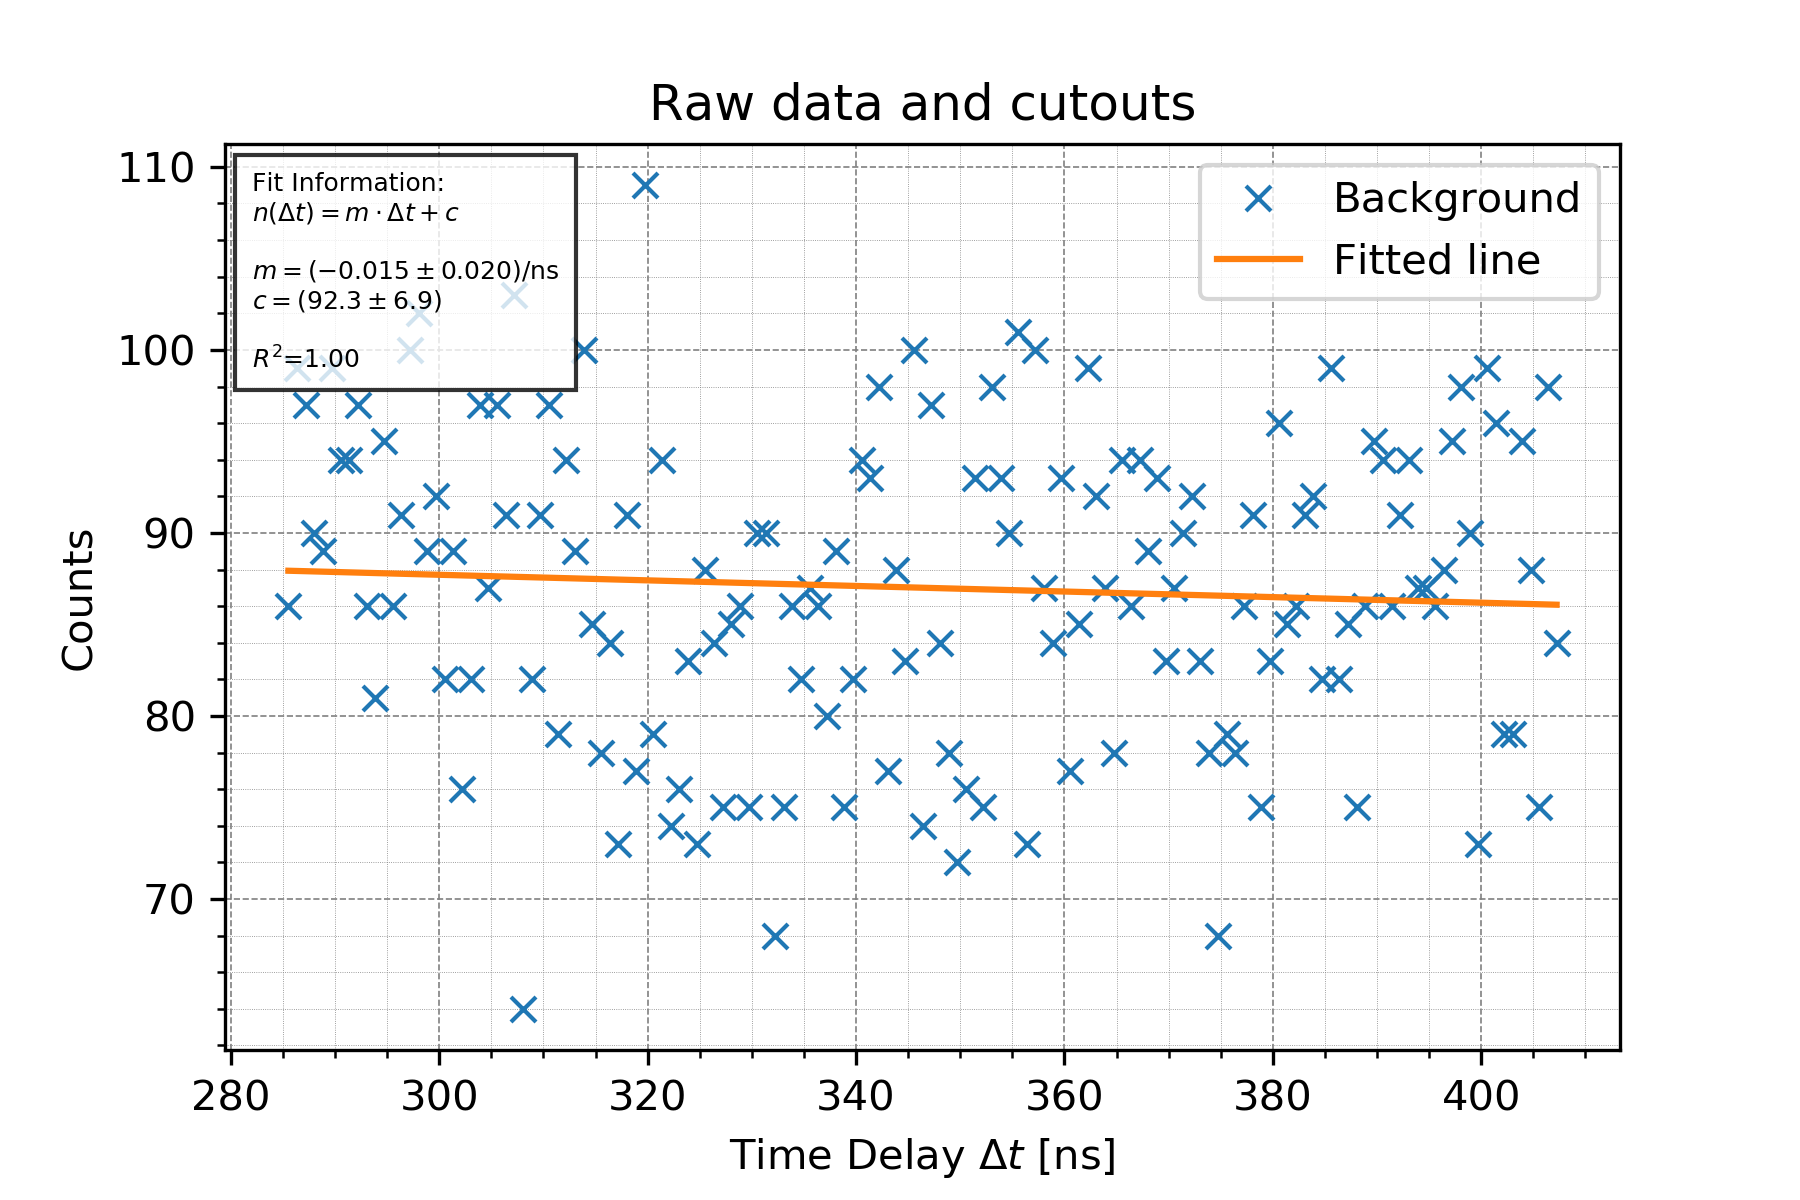
\includegraphics{Bilder/lin_bkgnd}
 		\centering
 		\caption{\small Plot of the datapoints with corrected time. The ranges of the data used for each different regression are marked in the graphic. The start and endpoints for each range are also given.}
 		\label{bckgnd_fit}
 	\end{figure}
 	
 	\FloatBarrier
 	After subtracting the background coincidences, a exponential function of the form
 	\ref{exp_style} was used to approximate the value of the decay constant $b$ in the fit. The parameter b in figure \ref{exp_fit} is the decay constant of our state. 
 	\begin{equation}
 	y\left(x,a,b,c,d\right) = a \cdot \exp\left(b\cdot\left(x+d\right)\right) + c
 	\label{exp_style}
 	\end{equation}
 	To get the half life the eq.\ref{Lifetime} can be used as well as eq.\ref{HalbwertszeitError} to calculate the error.
 	\begin{equation}
 	T_\frac{1}{2}=\frac{\log(2)}{b}
 	\label{Lifetime} 
 	\end{equation}
 	\begin{equation}
 	\Delta_T=\frac{\log(2)}{b^2}
 	\label{HalbwertszeitError} 
 	\end{equation}
 	With that the half life is $T_\frac{1}{2}=(83\pm10)$\,ns.
 	\begin{figure}[h]
 		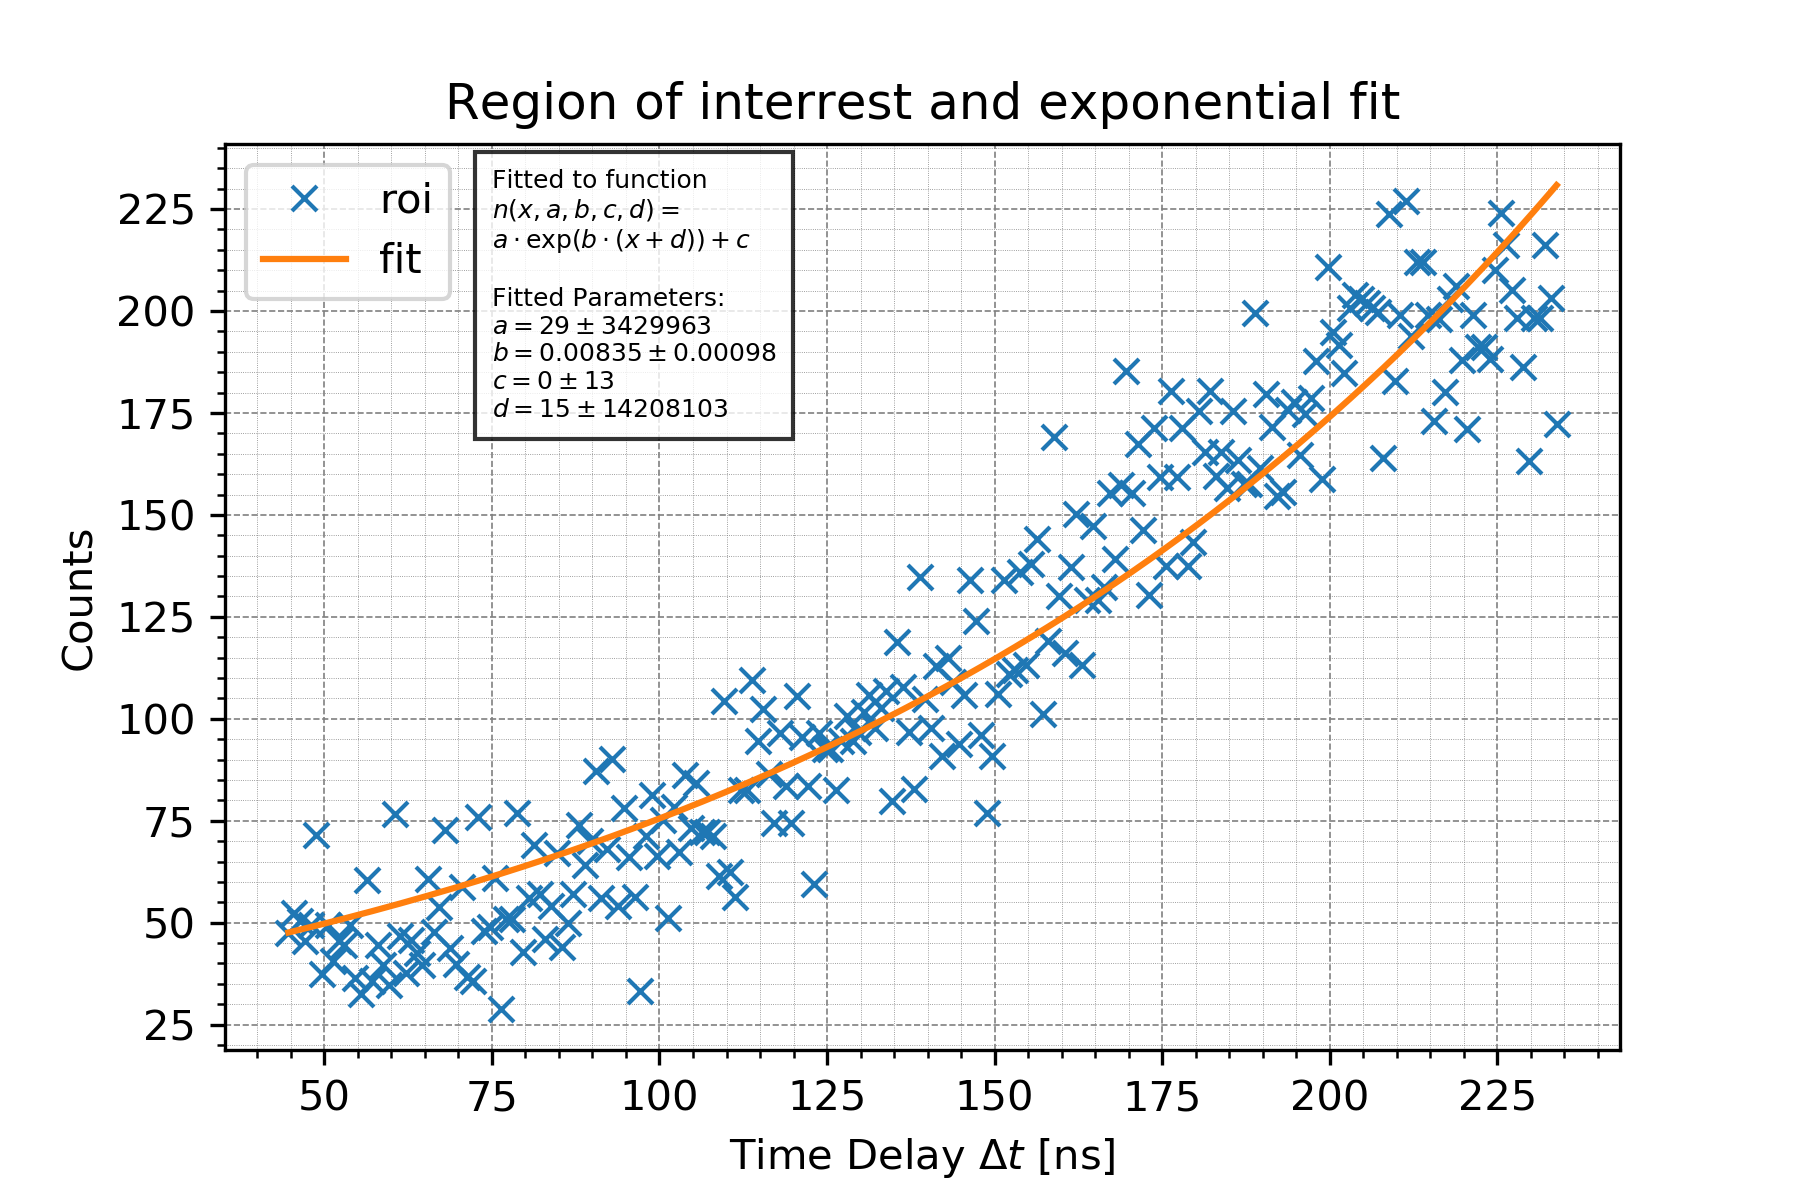
\includegraphics{Bilder/lin_fit_exp}
 		\centering
 		\caption{\small Plot of the datapoints in the roi with the fitted exponential curve. The determined parameters are given in the picture.}
 		\label{exp_fit}
 	\end{figure}
 	
 	\FloatBarrier
 	\bibliographystyle{plain}
 	\bibliography{Quellen}
 	\addcontentsline{toc}{section}{Literatur}
\end{document}